% SVN info for this file
\svnidlong
{$HeadURL$}
{$LastChangedDate$}
{$LastChangedRevision$}
{$LastChangedBy$}

\chapter{Il flusso del campo magnetico e la legge di Biot-Savart}
\labelChapter{leggeBiotSavart}

\begin{introduction}
	‘‘L’elettricità e il magnetismo sono quelle forze della natura grazie alle quali le persone che non sanno nulla di elettricità e magnetismo possono spiegare tutto.''
	\begin{flushright}
		\textscsl{Egon Friedell}, cercando di spiegare nulla.
	\end{flushright}
\end{introduction}
\lettrine[findent=1pt, nindent=0pt]{P}{er}  %TODO: intro

\section{Il flusso del campo magnetico per superfici aperte}
Come già detto, il campo magnetico è \textit{solenoidale}, ossia che la divergenza di esso è nulla:
\begin{equation*}
	\div{B}=0
\end{equation*}
Ne consegue che, almeno \textit{localmente}, esiste un vettore $\vba{A}$ detto \textbf{potenziale vettore}\index{potenziale!vettore} $\vba{A}$ tale per cui il campo magnetico è il gradiente di $\vba{A}$.
\begin{equation}
	\vba{B}=\curl{A}
\end{equation}
Questo ci viene in aiuto se vogliamo calcolare il flusso di $\vba{B}$ attraverso una superficie \textit{aperta} $\Sigma$ - per quelle chiuse sappiamo già che è nullo. Supponiamo che il bordo $\partial \Sigma$ sia una curva chiusa; allora
\begin{align*}
	\Phi_{\Sigma}(\vba{B})&=\int_{\Sigma}\vba{B}\vdot\vbh{u}_nd\Sigma=\\
	&=\int_{\Sigma}\left(\curl{\vba{A}}\right)\vdot\vbh{u}_nd\Sigma=&&\text{(}\vba{B}\ \text{solenoidale)}\\
	&=\int_{\partial \Sigma}\vba{A}\vdot d\vba{s}=\Gamma_{\Sigma}(\vba{A})&&\text{(teorema di Stokes)}
\end{align*}
Quanto trovato è valido in generale per un qualunque campo solenoidale: il flusso tramite una superficie aperta dipende esclusivamente dal \textit{bordo} e \textit{non} dalla superficie in sé. Se prendessi due superfici aperte differenti, ma con lo stesso bordo, avremmo lo stesso flusso.

Noto ciò, vorremmo ora \textit{generalizzare} ancora di più quanto visto nelle sezioni precedenti: dato un circuito qualunque percorso da corrente e immerso in un campo magnetico, vorremo esprimere la forza che agisce, l'energia potenziale, il lavoro del campo magnetico e quant'altro in termini di \textit{flusso}, in modo da utilizzare poi la dipendenza del flusso nei confronti del bordo.

Dato un circuito chiuso $\gamma$, scegliamo una superficie $\Sigma$ arbitraria con bordo $\partial \Sigma=\gamma$. Vorremmo calcolare il gradiente del flusso:
\begin{equation*}
	\grad{\Phi_\Sigma(\vba{B})}=\grad{\Gamma_{\partial\Sigma}(\vba{A})}
\end{equation*}
Invece che calcolare il gradiente della circuitazione vera e propria di $\vba{A}$, ossia
\begin{equation}
	\grad{\Gamma_{\partial\Sigma}(\vba{A})}=\grad{\int_{\partial\Sigma}\vba{A}\vdot d\vba{s}},
\end{equation}
ci conviene prima calcolare il gradiente della circuitazione \textit{infinitesima} $\vba{A}\vdot d\vba{s}$ per poi integrare lungo $\partial\Sigma$.
Si osservi che per il gradiente di un prodotto scalare tra vettori vale la formula per nulla immediata
\begin{equation}
	\grad{\vba{A}\vdot\vba{B}}=\left(\vba{A}\vdot\grad\right)\vba{B}+\left(\vba{B}\vdot\grad\right)\vba{A}+\vba{A}\cross\left(\grad\cross\vba{B}\right)+\vba{B}\cross\left(\grad\cross\vba{B}\right)
\end{equation}
Se consideriamo nel nostro caso come vettori $\vba{A}$ e lo spostamento infinitesimo $d\vba{s}$ della curva $\partial \Sigma$, otteniamo
\begin{equation*}
	\grad{\vba{A}\vdot d\vba{s}}=\left(\vba{A}\vdot\grad\right)d\vba{s}+\left(d\vba{s}\vdot\grad\right)\vba{A}+\vba{A}\cross\left(\grad\cross d\vba{s}\right)+d\vba{s}\cross\left(\grad\cross d\vba{s}\right)
\end{equation*}
Posta $\vba{r}$ la parametrizzazione di $\partial \Sigma$, si ha
\begin{equation*}
	\pdv{x} d\vba{s}=
	\pdv{y} d\vba{s}=
	\pdv{z} d\vba{s}=0
\end{equation*} %TODO: perchè scusi?
Noto che lo spostamento infinitesimo della curva $\partial \Sigma$ è
\begin{equation*}
	d\vba{s}=\dv{\vba{r}}{t}dt,
\end{equation*}
vale
\begin{equation*}
	\pdv{q^i} d\vba{s}=
	\pdv{q^i} \dv{\vba{r}}{t}dt=
	\dv{t} \pdv{\vba{r}}{q^i}dt=0
\end{equation*}
dove $q^1=x$, $q^2=y$, $q^3=z$.
Di conseguenza,
\begin{equation*}
	\begin{cases}
		\left(\vba{A}\vdot\grad\right)d\vba{s}=A_x\pdv{x} d\vba{s}+A_y\pdv{y} d\vba{s}+A_z\pdv{z} d\vba{s}=0\\
		\curl{d\vba{s}}=0
	\end{cases}
\end{equation*} %TODO: inserire curl esplicito
Ci interessano solo le derivate applicate al vettore potenziale $\vba{A}$:
\begin{equation*}
	\grad{\left(\vba{A}\cdot d\vba{s}\right)}=\left(d\vba{s}\vdot\grad\right)\vba{A}+d\vba{s}\cross\left(\grad\cross\vba{A}\right)
\end{equation*}
Calcoliamo la circuitazione di $\vba{A}$ facendo l'integrale curvilineo lungo il circuito $\partial \Sigma$:
+\begin{equation}
	\oint\grad{\left(\vba{A}\vdot d\vba{s}\right)}=\oint \left(d\vba{s}\vdot\grad\right)\vba{A}+\oint d\vba{s}\cross\left(\grad\cross\vba{A}\right)
\end{equation}
Osserviamo che, data una funzione scalare arbitraria $\oldphi$, vale
\begin{equation*}
	\left(d\vba{s}\vdot\grad\right)\phi=\pdv{\phi}{x}\pdv{x}{t}dt+\pdv{\phi}{y}\pdv{y}{t}dt+\pdv{\phi}{z}\pdv{z}{t}dt=\dv{t} \left(\phi(\vba{r}(t))\right)
\end{equation*}
e dunque
\begin{equation}
	d\vba{s}\vdot\grad=\left(\dv{\vba{r}}{t}\vdot\grad\right)dt
\end{equation}
Di conseguenza, $d\vba{s}\vdot\grad$ agisce su ciascuna componente di $\vba{A}$ come \textit{derivata totale} e di conseguenza, integrando su una curva chiusa, l'integrale risulta nullo; segue che il primo termine è nullo. Ricaviamo quindi
\begin{equation*}
	\grad{\Phi_{\Sigma}(\vba{B})}=\grad{\Gamma_{\partial \Sigma}(\vba{A})}=\oint d\vba{s}\cross\left(\grad\cross\vba{A}\right)=\oint d\vba{s}\cross\vba{B}
\end{equation*}
Ma quella che abbiamo ottenuta è la forza di Laplace divisa per l'intensità di corrente $I$ stazionaria. Nella condizione in cui $I$ sia stazionaria, allora
\begin{equation}
	\vba{B}=I\int_{\gamma}d\vba{s}\cross\vba{B}=I\grad{\Phi_{\Sigma}(\vba{B})}
\end{equation}
\paragraph{Energia potenziale}
Poiché la forza è espressa come \textit{gradiente} di una quantità scalare, l'energia potenziale è l'opposta di tale quantità:
\begin{equation}
	U_P=-I\Phi_{\Sigma}(\vba{B})
\end{equation}
In sintesi:
\begin{align}
	\vba{F}=&-\grad{U_P}\\
	U_P=&-I\Phi_{\Sigma}(\vba{B})
\end{align}
In particolare, se il campo magnetico $\vba{B}$ è uniforme, allora
\begin{align*}
	\Phi_{\Sigma}(\vba{B})&=\int_{\Sigma}\vba{B}\vdot\vbh{u}_nd\Sigma=\vba{B}\vdot\vbh{u}_n \Sigma\\
	&\implies U_P=I\Sigma \vbh{u}_n \vdot \vba{B}=-\vba{m}\vdot\vba{B}. 
\end{align*}
che, effettivamente, coincide con quanto abbiamo visto a pagina \pageref{EnergiaPotenzialeCasoGeneralemanontroppo}.
\paragraph{Lavoro per spostare il circuito}
Il circuito percorso da corrente, essendo soggetto alla forze di Laplace, si muove e si deforma. Ci si aspetterebbe di incontrare degli attriti, ma così non è, come mai?\\
Supponiamo che il campo magnetico $\vba{B}$ sposti un circuito lungo un percorso $\eta$ dallo stato $A$ allo stato $B$, deformandolo al contempo. Allo stato $A$ il circuito corrisponde alla curva $\gamma_A$, mentre allo stato $B$ alla curva $\gamma_B$. Il lavoro compiuto dal campo magnetico per spostare il circuito è
\begin{align*}
	W&=\int_{\eta}\vba{F}\vdot d\vba{s}=-\int_{\eta}\grad{U_P}\vdot d\vba{s}=&&\\
	&=-\Delta{U_P})=U_P(A)-U_P(B)&&\text{(teorema del gradiente)}
\end{align*}
dove $U_P(A)$ è il potenziale allo stato iniziale $A$ e $U_P(B)$ quello allo stato finale $B$. Oltre a non avere alcun attrito, dato che il lavoro è una differenza di energia potenziale senza dispersione, si ha anche che
\begin{equation}
	W=I(\Phi_{\Sigma_B}(\vba{B})-\Phi_{\Sigma_A}(\vba{B}))=I\left(\Gamma_{\gamma_B}(\vba{A})-\Gamma_{\gamma_A}(\vba{A})\right)
\end{equation}
dove $\Sigma_A,\ \Sigma_B$ sono superficie arbitrarie con bordo i circuiti $\gamma_A,\ \gamma_B$, rispettivamente.

Di fatto, il circuito elettrico è l'equivalente per il lavoro magnetostatico a quello che la particella elettrica fa nel lavoro elettromagnetico: alla carica corrisponde l'intensità di corrente, mentre alla differenza di potenziale corrisponde la differenza di circuitazione del potenziale vettore.

Per un campo magnetico uniforme sappiamo che la forza di Laplace su un circuito chiuso è \textit{nulla}, quindi anche il lavoro compiuto è \textit{nullo}.
\subsection{Un esempio: la spira circolare vicino al magnete cilindrico}
Consideriamo un \textit{magnete cilindrico} con asse lungo l'asse $z$; poniamo nello spazio una spira circolare $\gamma$, percorsa da corrente, in modo da essere parallela alla faccia orizzontale del magnete e tale per cui il centro della spira stia sull'asse $z$.
\begin{center}
	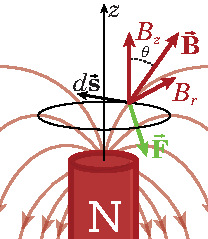
\includegraphics[width=0.4\textwidth]{images/chp8/chp8magnetecilindrico1.pdf}
\end{center}
Per ovvi motivi, poniamoci nelle coordinate cilindriche:
\begin{equation*}
	\begin{cases}
		x=R\sin\theta\\
		y=R\cos\theta\\
		z=z
	\end{cases}
\end{equation*}
Possiamo parametrizzare la spira di raggio $R=R_0$ e quota $z=z_0$ (inizialmente) fissati con
\begin{equation*}
	\vba{r}(\phi)=\left(x(\phi),y(\phi),z(\phi)\right)=\left(R_0\cos\phi,\ R_0\sin\phi, z_0\right)=
\end{equation*}
Uno spostamento infinitesimo in coordinate cilindriche sarebbe\footnote{	Nelle ‘‘XXX'', a pagina \pageref{spinfinitesimocilindriche} è possibile trovare come si calcola.}
\begin{equation}
	d\vba{s}=dR\vbh{u}_R+Rd\theta\vbh{u}_\theta+dz\vbh{u}_z
\end{equation}
Nel nostro caso, poiché $R=R_0$ e $z=z_0$ sono inizialmente fissi, si ha solo la variazione infinitesima $d\theta$ e quindi
\begin{equation}
	d\vba{s}=Rd\theta\vbh{u}_\theta
\end{equation}
Il campo magnetico $\vba{B}$ ha simmetria assiale rispetto all'asse $z$ e si può scomporre come
\begin{equation}
	\vba{B}=B\cos\phi\vbh{u}_z+B\sin\phi\vbh{u}_r
\end{equation}
dove $\phi$ è l'angolo tra l'asse $z$ e il campo. Calcoliamoci la forza: per la seconda legge di Laplace
\begin{equation*}
	\vba{F}=I\int d\vba{s}\cross\vba{B}
\end{equation*}
Per la regola della mano destra la forza sarà ortogonale sia a $d\vba{s}$ che a $\vba{B}$ e diretta verso il basso: in particolare, ci si aspetta che le componenti radiali di tali forze si compensino, in modo che la spira venga quindi ``risucchiata'' verso il basso senza deformarsi.
\begin{center}
	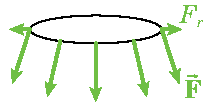
\includegraphics[width=0.35\textwidth]{images/chp8/chp8magnetecilindrico2.pdf}
\end{center}
Facendo i dovuti calcoli,
\begin{equation*}
	\vba{F}=I\int d\vba{s}\cross\vba{B}=IR\int\vbh{u}_{\theta}\cross\left(B\cos\phi\vbh{u}_z+B\sin\phi\vbh{u}_r\right)d\theta\squarequal
\end{equation*}
Poiché
\begin{align*}
	\vbh{u}_{\theta}\cross\vbh{u}_{z}=\vbh{u}_R&&
	\vbh{u}_{\theta}\cross\vbh{u}_{R}=\vbh{u}_z
\end{align*}
si ha
\begin{equation*}
	\squarequal IR\int \left(B\cos\phi\vbh{u}_R-B\sin\phi\vbh{u}_z\right)d\theta\squarequal
\end{equation*}
Osserviamo che per simmetria cilindrica lungo la spira $B$ e $\phi$ devono essere costanti, dunque anche $\cos\phi$ e $\sin\phi$ lo sono:
\begin{equation*}
	\squarequal IRB\cos\phi\int \vbh{u}_Rd\theta-B\sin\phi\int\vbh{u}_zd\theta
\end{equation*}
Si osservi che
\begin{itemize}
	\item $\displaystyle\int\vbh{u}_Rd\theta=0$. Ci sono due modi per convincersi che sia così: o per ragioni di simmetria, dato che ogni versore ha un versore opposto e quindi integrando su un giro completo dell'angolo $\theta$ si annullano tutti, oppure integrando il versore rispetto a $\theta$, noto che $\vbh{u}_R=\left(\cos\theta,\sin\theta\right)$. 
	\item $\displaystyle\int\vbh{u}_zd\theta=\vbh{u}_z\int d\theta=2\pi\vbh{u}_z$, dato che $\vbh{u}_z$ è costante.
\end{itemize}
Segue quindi che la forza subita dalla spira è diretta verso il basso, come previsto:
\begin{equation}
	\vba{F}=-2\pi R I B\sin\phi\vbh{u}_z
\end{equation}
Vorremmo ora esprimere questa forza come
\begin{equation*}
	\vba{F}=I\grad{\Phi_{\Sigma}(\vba{B})}
\end{equation*}
Per farlo, usiamo un trucco: consideriamo, in aggiunta alla spira circolare, un'altra spira \textit{immaginaria} posta ad altezza $\Delta z$; sfrutteremo che il flusso tramite questa superficie cilindrica individuata dalle spire è nullo. Indichiamo con
\begin{itemize}
	\item $\Sigma$ la superficie individuata dalla spira originale (base inferiore del cilindro).
	\item $\Sigma'$ la superficie individuata dalla spira immaginaria (la base superiore del cilindro).
	\item $\sigma$ la superficie laterale del cilindro.
\end{itemize}
Scegliamo un'orientazione di $\vbh{u}_n$ in modo che sia uscente dal cilindro.
\begin{center}
	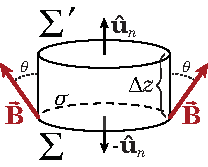
\includegraphics[width=0.35\textwidth]{images/chp8/chp8magnetecilindrico3.pdf}
\end{center}
% nelle note: il flusso della superficie attraversi il circuito nella stessa direzione sia sopra, sia sotto.
In questo caso, poniamo il versore normale di $\Sigma'$ nella direzione positiva dell'asse $z$ e quello di $\Sigma$ uguale e contrario. Allora
\begin{equation*}
	\Phi_{\Sigma+\Sigma'+\sigma}(\vba{B})=\Phi_{\Sigma'}(\vba{B})-\Phi_{\Sigma}(\vba{B})+\Phi_{\sigma}(\vba{B})=0
\end{equation*}
Il flusso relativo alle basi si può vedere una funzione della quota $z$:
\begin{equation*}
	\funztot[\Phi]{\realset}{\realset}{z}{\Phi(z)=\Phi_{\Sigma(z)}(\vba{B})}
\end{equation*}
dove $\Sigma(z)$ è l'area contenuta in una spira circolare di raggio $R_0$ a quota $z$. Allora:
\begin{align*}
	\Phi_{\Sigma}(\vba{B})=\Phi(z)&&\Phi_{\Sigma'}(\vba{B})=\Phi(z+\Delta z)
\end{align*}
Calcoliamo la derivata di tale funzione:
\begin{equation*}
	\pdv{\Phi_{\Sigma}}{z}=\lim_{\Delta z\to 0}\frac{\Phi_{\Sigma'}(\vba{B})-\Phi_{\Sigma}(\vba{B})}{\Delta z}=\lim_{\Delta z\to 0}\frac{-\Phi_{\sigma}(\vba{B})}{\Delta z}\squarequal
\end{equation*}
Si osservi che
\begin{align*}
	\Phi_{\sigma}(\vba{B})&=\int_{\sigma}\vba{B}\vdot\vbh{u}_nd\sigma=&&\\
	&=\int_{\sigma}B\vdot\vbh{u}_Rd\sigma=&&\text{(versore della sup. laterale)}\\
	&=\int_{\sigma}\left(B\cos\phi\vbh{z}+B\sin\phi\vbh{u}_R\right)\vdot\vbh{u}_Rd\sigma=&&\\
	&=\int_{\sigma}B\sin\phi d\sigma=&&\\
	&=B\sin\phi\int_{\sigma}d\sigma=&&\text{(}B\sin\phi\ \text{costante su}\ \sigma\ \text{per}\ \Delta z\to 0\text{)}\\
	&=2\pi R \Delta z B\sin\phi&&
\end{align*}
Si ottiene infine
\begin{equation*}
	\squarequal\lim_{\Delta z\to 0}\frac{-2\pi R \Ccancel[red]{\Delta z} B\sin\phi}{\Ccancel[red]{\Delta z}}=-2\pi R B\sin\phi
\end{equation*}
ossia
\begin{equation}
	\vba{F}=-2\pi IRB\sin\phi\vbh{u}_z=I\pdv{\Phi_{\Sigma}}{z}\vbh{u}_z
\end{equation}
\begin{observe}
	La forza dipende della variazione del flusso tramite l'area della spira; tuttavia, abbiamo appena mostrato che tale variazione si esprime in termini di flusso \textit{traverso}, cioè quello della \textit{superficie laterale}.
\end{observe}
\subsection{Unità di misura del flusso del campo magnetico}
L'unità di misura del flusso del campo magnetico si può derivare in diversi modi. Dalla definizione di flusso stesso, si ha
\begin{equation*}
	\left[\Phi_{\Sigma}(\vba{B})\right]=\left[\vba{B}\right]\left[\Sigma\right]=\unit[per-mode = fraction,exponent-product=\ensuremath{\cdot}]{\tesla\meter\squared}
\end{equation*}
Alternativamente, poiché il flusso è legato all'energia potenziale dalla legge
\begin{equation*}
	U_p=-I\Phi_{\Sigma}(\vba{B})
\end{equation*}
si ha anche
\begin{equation*}
	\left[\Phi_{\Sigma}(\vba{B})\right]=\frac{\left[U_P\right]}{\left[I\right]}=\unit[per-mode = fraction,exponent-product=\ensuremath{\cdot}]{\joule\per\ampere}
\end{equation*}
\begin{units}~\\
	\textbf{\textsc{Flusso magnetico:}} weber ($\unit{\weber}$).\\
	\textit{\textbf{Dimensioni:}} $\left[\Phi_{\Sigma}(\vba{B})\right]=\left[\vba{B}\right]\left[\Sigma\right]=\mathsf{M}\mathsf{L}^2 \mathsf{T}^{-2}  \mathsf{I}^{-1}$
\end{units}
\section{Prima legge di Laplace o legge di Biot-Savart}
L'esperimento di Ampère\footnote{Si veda la sezione \ref{EsperimentodiAmpere}, pag. \pageref{EsperimentodiAmpere}.} ci mostrò che due fili percorsi da corrente venivano attratti - o respinti - da forze di natura magnetica. Grazie alla forza di Lorentz ora sappiamo \textit{come} questi fili potevano muoversi: la corrente che percorre ciascun filo genera un campo magnetico che agisce sulle cariche in movimento dell'altro filo, le quali subiscono delle forze che, di conseguenza, permettono di spostarlo. Ci rimane un tassello di questo puzzle: qual è il campo magnetico \textit{generato dal filo}?

\subsection{Campo magnetico generato da cariche puntiformi in moto}
Procediamo con calma. Innanzitutto, sebbene sia difficilmente osservabile, anche una singola carica in movimento con velocità $\vba{v}$ è in grado generare un campo magnetico. Tale campo $\vba{B}$ soddisfa, nel suo piccolo, alcune proprietà incontrate nell'esperimento di Ampère:
\begin{itemize}
	\item Se la carica non è in movimento, non si ha alcun campo; dobbiamo supporre che $\vba{B}$ debba dipendere dalla velocità.
	\item Se il campo agisce su un'altra carica in movimento, la cui velocità ha direzione parallela a $\vba{v}$, la forza di Lorentz che ne consegue deve essere tale da risultare attrattiva se i versi delle velocità sono concordi e repulsiva se sono discordi. 
\end{itemize}
Fu \textbf{Oliver Heaviside} nel 1888 a derivare, dalle leggi di Maxwell, la legge matematica che descrive il campo magnetico generato da una singola carica in movimento:
\begin{equation}
	\vba{B}=\frac{\mu_0}{4\pi}\frac{q\vba{v}\cross\vbh{u}_r}{r^2}
\end{equation}
La prima cosa che notiamo è che, a tutti gli effetti, tale legge soddisfa quanto supposto ed osservato: il campo magnetico \textit{dipende} dalla velocità, mentre il prodotto vettoriale garantisce la seconda osservazione.

\begin{example}
	Per capire meglio la presenza del prodotto vettoriale consideriamo la seguente situazione: due particelle $1$ e $2$ in moto, entrambe con velocità $\vba{v}$ concorde e parallele, sono attratte l'un l'altra da forze di Lorentz  uguali e contrarie. La forza che subisce la particella $2$ è dovuta all'azione del campo magnetico $\vba{B}_1$ generato dalla prima.~\\
	\begin{minipage}{0.6\textwidth}
		\begin{equation*}
			\vba{F}_{2,1}=q_2\vba{v}_2\cross\vba{B}_1
		\end{equation*}
	Supponendo che le cariche siano negative, per avere che $\vba{F}_{2,1}$ sia attrattiva (cioè diretta verso la particella $1$), per la regola della mano destra $\vba{B}_1$ deve essere entrante il piano dove viaggiano le particelle. Allora, il prodotto vettoriale di $\vba{v}$ per il versore $\vbh{u}_r$ diretto dalla prima alla seconda carica permette a $vba{B}_1$ di avere verso entrante.
	\end{minipage}\hspace{5pt}
	\begin{minipage}{0.39\textwidth}
		\begin{center}
			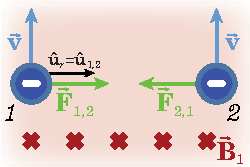
\includegraphics[width=0.9\textwidth]{images/chp8/chp8biotsavartcariche.pdf}
		\end{center}
	\end{minipage}
\end{example}
%TODO: check this, not so sure
\begin{observe}~\\
	\begin{minipage}{0.75\textwidth}
		Una carica in movimento genera sia un campo elettrico, sia un campo magnetico. In particolare, il campo elettrico si distribuisce \textit{radialmente} con centro la carica, mentre quello magnetico è \textit{tangenziale} a circonferenze \textit{perpendicolari} alla velocità e con centro sulla retta su cui essa giace.
	\end{minipage}\hspace{5pt}
	\begin{minipage}{0.24\textwidth}
			\begin{center}
			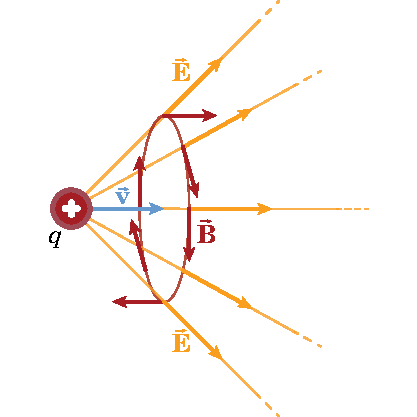
\includegraphics[width=0.75\textwidth]{images/chp8/chp8campomagneticoelettrico.pdf}
		\end{center}
	\end{minipage}
\end{observe}
Si noti che l'espressione del campo magnetico
\begin{equation*}
	\vba{B}=\frac{\mu_0}{4\pi}\frac{q\vba{v}\cross\vbh{u}_r}{r^2}
\end{equation*}
e quella del campo elettrico
\begin{equation*}
	\vba{E}=\frac{1}{4\pi\epsilon_0}\frac{q}{r^2}\vbh{u}_r
\end{equation*}
generati della particella sono così simili da essere collegati tra di loro dalla relazione
\begin{equation}
	\vba{B}=\mu_0\epsilon_0\vba{v}\cross\vba{E}
\end{equation}
Poiché, dimensionalmente parlando, si ha
\begin{equation*}
	\left[\epsilon_0\right]=\frac{1}{4\pi\left[F\right]}\frac{\left[q\right]^2}{\left[r\right]^2}=\unit[per-mode = fraction]{\coulomb\squared\per\meter\squared\per\newton}
\end{equation*}
e
\begin{equation*}
	\left[\mu_0\right]=\unit[per-mode = fraction]{\newton\second\squared\per\coulomb\squared},
\end{equation*}
il loro prodotto ha dimensioni
\begin{equation*}
	\left[\epsilon_0\mu_0\right]=\unit[per-mode = fraction]{\second\squared\per\meter\squared},
\end{equation*}
pari a quelle di un inverso di un quadrato di una velocità. Ma non stiamo parlando di una velocità qualunque, bensì della \textit{velocità della luce}! Infatti,
\begin{equation*}
	c=\SI[per-mode = fraction]{3d8}{\meter\per\second}=\frac{1}{\sqrt{\epsilon_0\mu_0}}
\end{equation*}
La relazione di cui sopra tra campo elettrico $\vba{E}$ e campo magnetico $\vba{B}$ di una particella carica in moto a velocità $\vba{v}$ si riscrive quindi come
\begin{equation}
	\vba{B}=\frac{1}{c^2}\vba{v}\cross\vba{E}
\end{equation}
Perché però compare la velocità della luce? Facendo un piccolissimo spoiler, i fenomeni elettromagnetici sono legati a fenomeni di natura ondulatoria con velocità di propagazione pari a quelli della luce.
\subsection{Campo magnetico generato da un filo: legge di Biot-Savart}
Sebbene abbiamo visto cosa succede per una particella, una singola carica in movimento non fa una corrente stazionaria - ma tante sì. Supponiamo di avere un elemento di filo infinitesimo percorso da corrente stazionaria di intensità $I$; le cariche si spostano con velocità di deriva $\vba{v}_d$. Per ciascuna singola carica il campo magnetico generato è
\begin{equation}
	\vba{B}_i=\frac{\mu_0}{4\pi}\frac{e\vba{v}_d\cross\vbh{u}_r}{r^2}
\end{equation}
Se nel volumetto ci sono $N$ cariche, si ha una densità di cariche pari a
\begin{equation*}
	n=\frac{dN}{dV}
\end{equation*}
Se sommiamo - con continuità - rispetto a tutte le cariche nel volumetto, il campo magnetico complessivo sarà dato da
\begin{equation*}
	\vba{B}=\frac{\mu_0}{4\pi}\int_V\frac{e\vba{v}_d\cross\vbh{u}_r}{r^2}dN=\frac{\mu_0}{4\pi}\int_V\frac{ne\vba{v}_d\cross\vbh{u}_r}{r^2}dV
\end{equation*}
Ricordando che $\vba{j}=ne\vba{v}_d$, allora
\begin{equation*}
	\vba{B}=\frac{\mu_0}{4\pi}\int_V\frac{\vba{j}\cross\vbh{u}_r}{r^2}dV
\end{equation*}
% bla bla bla confronto con il campo elettrico
Consideriamo il caso di un filo rettilineo  $\mathcal{l}$: un suo volumetto infinitesimo ha spessore costante $d\Sigma$ e lunghezza $ds$. Se poniamo il filo lungo l'asse $x$ senza perdita di generalità, la densità di corrente è anch'essa parallela all'asse $x$, ossia
\begin{equation*}
	\vba{j}=j\vbh{u}_x
\end{equation*}
Il campo magnetico sarà
\begin{equation*}
	\vba{B}=\frac{\mu_0}{4\pi}\int_V\frac{\vba{j}\cross\vbh{u}_r}{r^2}d\Sigma ds=\frac{\mu_0}{4\pi}\int_{\mathcal{l}}j\Sigma\frac{\vbh{u}_x\cross\vbh{u}_r}{r^2}=\frac{\mu_0}{4\pi}\int_{\mathcal{l}}I\frac{\vbh{u}_x\cross\vbh{u}_r}{r^2}ds
\end{equation*}
Osserviamo che in questo caso $d\vba{s}=ds\vbh{u}_x$. Generalizziamo quanto trovato.

\begin{define}[Seconda legge di Laplace]
	La \textbf{legge di Biot-Savart}\index{legge!di Biot-Savart}, detta anche \textbf{prima legge di Laplace}\index{legge!di Laplace!prima}, afferma che il campo magnetico indotto da una corrente stazionaria $I$ che percorre un filo descritto dalla curva $\gamma$ è pari a
	\begin{equation}
		\vba{B}=\frac{\mu_0}{4\pi}\int_{\gamma}\frac{d\vba{s}\cross\vbh{u}_r}{r^2}
	\end{equation}
	dove $d\vba{s}$ è lo spostamento infinitesimo lungo la curva $\gamma$ e $\vbh{u}_r$ il versore dal tratto di filo al punto in cui viene valutato il campo magnetico. 
\end{define}
\begin{observe}
	Per sapere il verso di $\vba{B}$ si può applicare la regola della vite destra: indicando con il pollice destro il verso della corrente, le dita della mano curvano seguendo le linee di campo del campo magnetico $\vba{B}$.
\end{observe}
\subsection{Campo magnetico generato da un filo rettilineo (in)finito}
Consideriamo un filo rettilineo di lunghezza $2a$, posto lungo l'asse $z$ in modo che il suo punto medio coincida con l'origine. La parametrizzazione di tale filo è data da
\begin{equation*}
	\vba{r}'=\left(0,0,z'\right)
\end{equation*}
da cui segue lo spostamento infinitesimo
\begin{equation*}
	d\vba{s}=dz'\vbh{u}_z
\end{equation*}
Il versore $\vbh{u}_r$ da un generico punto sul filo verso un punto generico $\vba{r}=(x,y,z)$ è
\begin{equation*}
	\vbh{u}_r=\frac{\vba{r}-\vba{r}'}{\abs{\vba{r}-\vba{r}'}}=\frac{\left(x,y,z-z'\right)}{\sqrt{x^2+y^2+\left(z-z'\right)^2}}
\end{equation*}
Calcoliamo
\begin{equation*}
	d\vba{s}\cross\vbh{u}_r=\frac{1}{\sqrt{x^2+y^2+\left(z-z'\right)^2}}
	\begin{vmatrix}
		0 & 0 & dz'\\
		x & y & z-z'\\
		\vbh{u}_x & \vbh{u}_y & \vbh{u}_z 
	\end{vmatrix}
	=\frac{x\vbh{u}_y-y\vbh{u}_x}{\abs{\vba{r}-\vba{r}'}}dz'
\end{equation*}
Il campo magnetico, per la legge di Biot-Savart, sarà
\begin{equation}
	\vba{B}=\frac{\mu_0 I}{4\pi}\int_{-a}^{a} \frac{x\vbh{u}_y-y\vbh{u}_x}{\left(x^2+y^2+\left(z-z'\right)^2\right)^{\nicefrac{3}{2}}}dz'
\end{equation}
Osserviamo però che il problema presentava un'evidente simmetria cilindrica. Passando alle coordinate cilindriche
\begin{equation*}
	\begin{cases}
		x=R\sin\theta\\
		y=R\cos\theta\\
		z=z
	\end{cases}
\end{equation*}
si ha
\begin{equation*}
	x\vbh{u}_y-y\vbh{u}_x=R\left(\sin\theta,\cos\theta\right)=R\vbh{u}_{\theta}
\end{equation*}
e noto che $x^2+y^2=R^2$, riscriviamo
\begin{equation*}
	\vba{B}=\frac{\mu_0 I}{4\pi}R\vbh{u}_{\theta}\int_{-a}^{a}\frac{dz'}{\left(R^2+\left(z-z'\right)^2\right)^{\nicefrac{3}{2}}}
\end{equation*}
Per semplicità, consideriamo un punto $\vba{r}$ con quota prossima a $0$ (cioè $z\to 0$). Allora
\begin{equation*}
	\vba{B}=\frac{\mu_0 I}{4\pi}R\vbh{u}_{\theta}\int_{-a}^{a}\frac{dz'}{\left(R^2+(z')^2\right)^{\nicefrac{3}{2}}}=\frac{\mu_0 I}{4\pi}R\vbh{u}_{\theta}\int_{-a}^{a}\frac{dz'}{R^3\left(1+(\frac{z'}{R})^2\right)^{\nicefrac{3}{2}}}\squarequal
\end{equation*}
Imponendo la sostituzione $b=\dfrac{z'}{R}$, il differenziale risulta $db=\dfrac{1}{R}dz'$ e gli estremi diventano $\pm\frac{a}{R}$; quindi
\begin{align*}
	&\squarequal\frac{\mu_0 I}{4\pi}\Ccancel[red]{R}\vbh{u}_{\theta}\int_{-\nicefrac{a}{R}}^{\nicefrac{a}{R}}\frac{\Ccancel[red]{R}db}{R^{\Ccancel[red]{3}}\left(1+b^2\right)^{\nicefrac{3}{2}}}=\\
	&=\frac{\mu_0 I}{4\pi R}\vbh{u}_{\theta}\eval{\frac{b}{\sqrt{1+b^2}}}_{-\nicefrac{a}{R}}^{\nicefrac{a}{R}}=\frac{\mu_0 I}{2\pi R}\frac{\nicefrac{a}{R}}{\sqrt{1+\frac{a^2}{R^2}}}\vbh{u}_{\theta}=\frac{\mu_0 I}{2\pi R}\frac{a}{\sqrt{a^2+R^2}}\vbh{u}_{\theta}
\end{align*}
Se facessimo tendere il valore di $a$ a $+\infty$, e cioè nel caso in cui filo fosse di \textit{lunghezza infinita}, il campo magnetico sarebbe descritta da quella che è la \textit{legge di Biot-Savart per un filo infinito}\index{legge!di Biot-Savart!per un filo infinito}:
\begin{equation}
	\vba{B}=\frac{\mu_0 I}{2\pi R}\vbh{u}_{\theta}
\end{equation}
Grazie a ciò siamo in grado di derivare per via teorica (e non più soltanto empirica) la legge di Ampère. Prendiamo i nostri due fili paralleli di lunghezza infinita. Il campo generato dal filo 1 in un punto sul secondo filo, posto a distanza $d$, è
\begin{equation*}
	\vba{B}_1=\frac{\mu_0 I_1}{2\pi d}\vbh{u}_\theta
\end{equation*}
La forza che agisce sul filo 2 su un tratto $\gamma_2$ di lunghezza $L$ è, per la seconda legge di Laplace, data da
\begin{equation*}
	\vba{F}_2=I_2\int_{\gamma_2}d\vba{s}\cross\vba{B}_1=I_2\left(\int_{\gamma_2}d\vba{s}\right)\cross\vba{B}_1=I_2\left(\int_{0}^Ldz\right)\vbh{u}_z\cross\vba{B}_1=I_2L\vbh{u}_z\cross\vba{B}_1
\end{equation*}
Da ciò concludiamo che 
\begin{equation*}
	\frac{\vba{F}_2}{L}=I_2\vbh{u}_z\cross\vba{B}_1=\frac{\mu_0 I_1 I_2}{2\pi d}\vbh{u}_z\cross\vbh{u}_{\theta}=\frac{\mu_0}{2\pi}\frac{I_1I_2}{d}\vbh{u}_d
\end{equation*}
Per simmetria, lo stesso risultato si ottiene considerando la forza che agisce sul filo 1 con il campo magnetico generato da 2, quindi
\begin{equation}
	\frac{\vba{F}}{L}=\frac{\mu_0}{2\pi}\frac{I_1I_2}{d}\vbh{u}_d
\end{equation}
\subsection{Campo magnetico generato da una spira circolare}
Consideriamo un circuito circolare in cui circola corrente. Per la legge di Biot-Savart, è presente un campo magnetico tangenziale a circonferenze perpendicolari alla corrente e centrate lungo il circuito, il cui verso è dato dalla legge della mano destra. Di conseguenza, ci aspettiamo un campo a simmetria cilindrica come in figura.
\begin{center}
	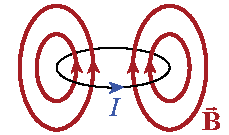
\includegraphics[width=0.4\textwidth]{images/chp8/chp8spiracampomagnetico.pdf}
\end{center}
Geometricamente parlando, la spira di raggio $R_0$ e posta nel piano $xy$ è una curva parametrizzabile da un angolo $\phi$:
\begin{equation*}
	\vba{r}'\left(\phi\right)=\left(R_0\cos\phi,R_0\sin\phi,0\right)
\end{equation*}
Lo spostamento infinitesimo lungo il circuito è quindi
\begin{equation*}
	d\vba{s}=\dv{\vba{r}'\left(\phi\right)}{\phi}d\phi=\left(-R_0\sin\phi,R_0\cos\phi,0\right)
\end{equation*}
Il versore $\vbh{u}_r$ da un generico punto sul filo verso un punto $\vba{r}=\left(R\cos\theta,R\sin\theta,z\right)$ nello spazio è
\begin{equation*}
	\vbh{u}_r=\frac{\vba{r}-\vba{r}'(\phi)}{\abs{\vba{r}-\vba{r}'(\phi)}}=\frac{\left(R\cos\theta-R_0\cos\phi,R\sin\theta-R_0\cos\theta,z\right)}{\sqrt{R^2+z^2+R_0^2-2RR_0\cos\left(\theta-\phi\right)}}
\end{equation*}
Calcoliamo
\begin{align*}
	d\vba{s}\cross\vbh{u}_r&=\frac{1}{\sqrt{R^2+z^2+R_0^2-2RR_0\cos\left(\theta-\phi\right)}}
	\begin{vmatrix}
		-R_0\sin\phi & R_0\cos\phi & 0\\
		R\cos\theta-R_0\cos\phi & R\sin\theta-R_0\cos\theta & z\\
		\vbh{u}_x & \vbh{u}_y & \vbh{u}_z 
	\end{vmatrix}
	=\\
	&=\frac{zR_0\cos\phi\vbh{u}_x+zR_0\sin\phi\vbh{u}_y+\left(R_0^2-RR_0\cos\left(\theta-\phi\right)\right)\vbh{u}_z}{\sqrt{R^2+z^2+R_0^2-2RR_0\cos\left(\theta-\phi\right)}}
\end{align*}
Il campo di induzione magnetica descritto dalla legge di Biot-Savart è
\begin{align*}
	\vba{B}&=\frac{\mu_0 I}{4\pi }\int_{\gamma}\frac{d\vba{s}\cross\vbh{u}_r}{r^2}=\frac{\mu_0 I}{4\pi}\int_{\gamma}{\abs{\vba{r}-\vba{r}'(\phi)}}=\\
	&=\frac{\mu_0 I}{4\pi }\int_0^{2\pi}d\phi\ \frac{zR_0\cos\phi\vbh{u}_x+zR_0\sin\phi\vbh{u}_y+\left(R_0^2-RR_0\cos\left(\theta-\phi\right)\right)\vbh{u}_z}{\left(R^2+z^2+R_0^2-2RR_0\cos\left(\theta-\phi\right)\right)^{\nicefrac{3}{2}}}
\end{align*}
Operando un cambio di variabile $\phi'=\phi-\theta$, osserviamo che
\begin{align*}
	\cos\phi\vbh{u}_x+\sin\phi\vbh{u}_y&=\cos\left(\phi'+\theta\right)\vbh{u}_x+\sin\left(\phi'+\theta\right)\vbh{u}_y=\\
	&=\left(\cos\theta\cos\phi'-\sin\theta\sin\phi'\right)\vbh{u}_x+\left(\cos\theta\sin\phi'+\sin\theta\cos\phi'\right)\vbh{u}_y=\\
	&=\cos\phi'\left(\cos\theta\vbh{u}_x+\sin\theta\vbh{u}_y\right)+\sin\phi'\left(-\sin\theta\vbh{u}_x+\cos\theta\vbh{u}_y\right)\squarequal
\end{align*}
Ricordando che
\begin{equation*}
	\begin{cases}
		\vbh{u}_R=\cos\theta\vbh{u}_x+\sin\theta\vbh{u}_y\\
		\vbh{u}_{\theta}=-\sin\theta\vbh{u}_x+\cos\theta\vbh{u}_y
	\end{cases}
\end{equation*}
si ha
\begin{equation*}
	\squarequal \cos\phi'\vbh{u}_R+\sin\phi'\vbh{u}_\theta
\end{equation*}
Allora il campo si può riscrivere come
\begin{equation*}
	\vba{B}=\frac{\mu_0 I}{4\pi }\int_0^{2\pi}d\phi'\ \frac{zR_0\left(\cos\phi'\vbh{u}_R+\sin\phi'\vbh{u}_\theta\right)+\left(R_0^2-RR_0\cos\phi'\right)\vbh{u}_z}{\left(R^2+z^2+R_0^2-2RR_0\cos\phi'\right)^{\nicefrac{3}{2}}}
\end{equation*}
Poniamo per compattezza di scrittura $A\coloneqq R^2+z^2+R_0^2$. Spezziamo il campo rispetto alle direzioni dell coordinate cilindriche:
\begin{itemize}
	\item \textit{Rispetto a }$\vbh{u}_{\theta}$:
	\begin{equation*}
		B_\theta=\frac{\mu_0 I}{4\pi }\int_0^{2\pi}d\phi'\frac{zR_0\sin\phi'}{\left(A-2RR_0\cos\phi'\right)^{\nicefrac{3}{2}}}=0
	\end{equation*}
	Questo vale perché l'integranda è dispari e stiamo integrando su un suo periodo; si può vedere anche più approfonditamente per sostituzione.
	\item \textit{Rispetto a} $\vbh{u}_{R}$:
	\begin{equation*}
		B_R=\frac{\mu_0 I}{4\pi }\int_0^{2\pi}d\phi'\frac{zR_0\phi'}{\left(A-2RR_0\cos\phi'\right)^{\nicefrac{3}{2}}}=0
	\end{equation*}
	Questo invece è un'integrale ellittico e non è elementarmente integrabile.
	\item \textit{Rispetto a} $\vbh{u}_z$: segue una situazione analoga a $\vbh{u}_R$.
\end{itemize}
Data l'evidente difficoltà della situazione in cui siamo incappati, vediamo solamente dei casi specifici di ciò.
\begin{itemize}
	\item \textbf{Asse della spira.} In questo caso $R=0$.
	\begin{align*}
		\vba{B}&=\frac{\mu_0 I}{4\pi }\int_0^{2\pi}d\phi'\ \frac{zR_0\cos\phi'\vbh{u}_R+R_0^2\vbh{u}_z}{\left(z^2+R_0^2\right)^{\nicefrac{3}{2}}}=\\
		&=\frac{\mu_0 I}{4\pi \left(z^2+R_0^2\right)^{\nicefrac{3}{2}}}\left[\vbh{u}_R\underbrace{\int_0^{2\pi}d\phi'\ zR_0\cos\phi'}_{=0} + \vbh{u}_z \int_0^{2\pi}d\phi'\ R_0^2d\phi'\right]=\\
		&=\frac{\mu_0 I R_0^2}{2 \left(z^2+R_0^2\right)^{\nicefrac{3}{2}}}\vbh{u}_z
	\end{align*}
	\begin{equation}
		\vba{B}=\frac{\mu_0 I R_0^2}{2 \left(z^2+R_0^2\right)^{\nicefrac{3}{2}}}\vbh{u}_z
	\end{equation}
	Il campo magnetico è verticale. In particolare, ha il suo massimo nel centro della spira ($z=0$), dove è pari a
	\begin{equation}
		\vba{B}=\frac{\mu_0 I}{2R_0}\vbh{u}_z
	\end{equation}
\end{itemize}
\begin{observe}
	Per capire il verso del campo magnetico lungo l'asse della spira vale un'altra versione \textbf{legge della vite destra}: curvando le dita della mano lungo la direzione della corrente, il pollice indicherà il verso del campo magnetico.\\
	Ad esempio, se la spira è percorsa in senso antiorario dalla corrente, allora il campo sarà diretto verso l'alto; viceversa se il circuito è percorso in senso orario.
\end{observe}
\begin{itemize}
	\item $\mathbf{R_0\ll r.}$ I casi sono due: o la spira è molto molto piccola, oppure stiamo osservando il campo a debita distanza da essa. In ogni caso la spira è assimilabile ad un \textit{punto}; per questo, passiamo dalle coordinate cilindriche alle coordinate sferiche. Se $r$ è la distanza dalla spira e $\theta$ l'angolo polare\footnote{Piccola ripetizione (qualcheduno direbbe \textit{abuso}) di notazione: abbiamo già usato $\theta$ in precedenza per l'angolo azimutale delle cilindriche, ma dato che in precedenza abbiamo fatto una sostituzione con $\phi'$ tale angolo non si ripresenta qui.}, allora 
	\begin{equation*}
		\begin{cases}
			R=r\sin\theta\\
			z=r\cos\theta
		\end{cases}
	\end{equation*}
	Possiamo anche esprimere i versori $\vbh{u}_R$ e $\vbh{u}_z$ delle coordinate cilindriche in funzione di quelli sferici $\vbh{u}_{\theta}$ e $\vbh{u}_r$ tramite una rotazione di essi (in senso orario) rispetto all'angolo polare:
	\begin{equation*}
		\begin{cases}
			\vbh{u}_R=\cos\theta\vbh{u}_{\theta}+\sin\theta\vbh{u}_{z}\\
			\vbh{u}_z=-\sin\theta\vbh{u}_{\theta}+\cos\theta\vbh{u}_{z}
		\end{cases}
	\end{equation*}
	Allora, facendo le opportune sostituzioni - e raccogliendo un fattore $r^2$ - otteniamo
	\begin{align*}
		\vba{B}&=\frac{\mu_0 I}{4\pi }\int_0^{2\pi}d\phi'\ \frac{R_0r\cos\theta\cos\phi'\vbh{u}_R+\left(R_0^2-R_0r\sin\theta\cos\phi'\right)\vbh{u}_z}{\left(r^2+R_0^2-2R_0r\sin\theta\cos\phi'\right)^{\nicefrac{3}{2}}}=\\
		&=\frac{\mu_0 I}{4\pi r}\int_0^{2\pi}d\phi'\frac{\frac{R_0}{r}\cos\phi'\vbh{u}_{\theta}+\frac{R_0^2}{r^2}\left(\cos\theta\vbh{u}_r-\sin\theta\vbh{u}_\theta\right)}{\left(1-2\frac{R_0}{r}\sin\theta\cos\phi'+\frac{R_0^2}{r^2}\right)^{\nicefrac{3}{2}}}
	\end{align*}
	Poiché $R_0\ll r$, approssimiamo in serie di Taylor rispetto a $\frac{R_0}{r}$ il denominatore fino all'ordine quadratrico.
	\begin{align*}
		\vba{B}\simeq&\frac{\mu_0 I}{4\pi r}\underbrace{\int_0^{2\pi}d\phi'\frac{R_0}{r}\cos\phi'}_{=0}\vbh{u}_{\theta}+\frac{R_0^2}{r}\left(\cos\theta\vbh{u}_r-\sin\theta\vbh{u}_\theta+3\cos^2\phi'\sin\theta\vbh{u}_\theta\right)=\\
		&=\frac{\mu_0 I}{4\pi r^3}\left(2\cos\theta\vbh{u}_r-2\sin\theta\vbh{u}_{\theta}+3\int_{0}^{2\pi}d\phi'\ \cos^2\phi'\ \sin\theta\vbh{u}_\theta\right)=\\
		&=\frac{\mu_0 I R_0^2}{4\pi r^3}\left(2\pi\cos\theta\vbh{u}_r-2\pi \sin\theta\vbh{u}_{\theta}+3\pi \sin\theta\vbh{u}_\theta\right)=\\
		&=\frac{\mu_0 I R_0^2 \pi}{4 \pi r^3}\left(2\cos\theta\vbh{u}_r+ \sin\theta\vbh{u}_\theta\right)
	\end{align*}
	Ricordiamo che il momento di dipolo magnetico è
	\begin{equation*}
		\vba{m}=I\Sigma\vbh{u}_n
	\end{equation*}
	dove $\Sigma$ è l'area della spira e $\vbh{u}_n$ il versore normale ad essa. Nel nostro caso
	\begin{equation*}
		\vba{m}=IR_0^2\pi\vbh{u}_z
	\end{equation*}
	Allora il campo magnetico, a debita distanza, è approssimabile da
	\begin{equation}
		\vba{B}=\frac{\mu_0 m}{4 \pi r^3}\left(2\cos\theta\vbh{u}_r+ \sin\theta\vbh{u}_\theta\right)
	\end{equation}
	\begin{example}
		Sul piano della spira, il campo magnetico lontano dalla spira punta verso il basso.
	\end{example}
	Si può anche scrivere come
	\begin{equation}
		\vba{B}=\frac{\mu_0}{4 \pi r^3}\left(3\left(\vba{m}\vdot\vbh{u}_r\right)\vbh{u}_z-\vba{m}\right)
	\end{equation}
\end{itemize}
\paragraph{Confronto con il dipolo elettrico}
\begin{center}
	\begin{tabular}{p{0.49\textwidth}p{0.49\textwidth}}
		\multicolumn{1}{c|}{\textbf{Dipolo elettrico}} &
		\multicolumn{1}{c}{\textbf{Spira circolare}} \\ \hline
				\multicolumn{2}{c}{\textbf{Momento}}\\\hline
				\multicolumn{1}{c|}{$\displaystyle\vba{p}=q\vba{a}$} & \multicolumn{1}{c}{$\displaystyle\vba{m}=I\Sigma\vbh{u}_n$}\\
				\multicolumn{1}{p{0.49\textwidth}|}{A grandi distanze non si distingue la \textit{distanza} dalla \textit{carica}, ma si può sapere solo il loro \textit{prodotto}.} & 
				A grandi distanze non si distingue la \textit{superficie} dall'\textit{intensità di corrente}, ma si può sapere solo il loro \textit{prodotto}.
				\\ \hline
				\multicolumn{2}{c}{\textbf{Campo generato}}\\\hline
				\multicolumn{1}{c|}{
					$\displaystyle\vba{E}=\frac{1}{4\pi\epsilon_0r^3}\left(3\left(\vba{p}\vdot\vbh{u}_r\right)\vbh{u}_z-\vba{p}\right)$
				} &
				\multicolumn{1}{c}{
					$\displaystyle\vba{B}=\frac{\mu_0}{4\pi r^3}\left(3\left(\vba{m}\vdot\vbh{u}_r\right)\vbh{u}_z-\vba{m}\right)$
				}\\
				\multicolumn{1}{c|}{Decade di un fattore $\nicefrac{1}{r^3}$.} & 
				\multicolumn{1}{c}{Decade di un fattore $\nicefrac{1}{r^3}$.}
				\\ \hline
				\multicolumn{2}{c}{\textbf{Momento subito torcente}}\\\hline
				\multicolumn{1}{c|}{
					$\displaystyle\vba{M}=\vba{p}\cross\vba{E}$
				} &
				\multicolumn{1}{c}{
					$\displaystyle\vba{M}=\vba{m}\cross\vba{B}$
				}\\ \hline
				\multicolumn{2}{c}{\textbf{Energia potenziale}}\\\hline
				\multicolumn{1}{c|}{
					$\displaystyle U=-\vba{p}\vdot\vba{E}$
				} &
				\multicolumn{1}{c}{
					$\displaystyle U=-\vba{m}\vdot\vba{B}$
				}\\ \hline
				\multicolumn{2}{c}{\textbf{Posso separare le ‘‘cariche''?}}\\\hline
				\multicolumn{1}{c|}{
					Sì.
				} &
				\multicolumn{1}{c}{
					No.
				}\\ \hline
			\end{tabular}
		\end{center}
		\begin{observe}
			Ci potrebbe capitare di dover studiare un campo elettrico senza sapere di preciso \textit{cosa} lo ha generato - se fosse una carica singola, oppure un dipolo, o un tripolo... Per capire meglio, si può sviluppare in serie di Taylor rispetto a $\frac{1}{r}$ il campo elettrico, in modo da ottenere una scrittura del genere
			\begin{equation*}
				\vba{E}=\frac{q}{4\pi \epsilon_0 r^2}\vbh{u}_r+\frac{3\left(\vba{p}\vdot \vbh{u}_r\right)\vbh{u}_r-\vba{p}}{4\pi\epsilon_0r^3}+\ldots+o\left(\frac{1}{r^n}\right)
			\end{equation*}%TODO: controllare
			A grandi distanze ($r\to+\infty$), prevale sempre il \textit{campo di monopolo} - che altro non è che quello \textit{di Coulomb}. Tuttavia, se \textit{non} abbiamo una carica - ad esempio nel caso del dipolo in cui le cariche si compensano tra di loro - allora prevale il secondo termine, il \textit{campo di dipolo}; se non abbiamo neanche un momento di dipolo prevarrà \textit{quello di tripolo} e cosi via.\\
			Si può fare una cosa analoga nel caso del campo magnetico. La differenza sostanziale, tuttavia, è che per quanto abbiamo visto \textit{non} c'è il termine di monopolo perché non esiste la carica magnetica.
		\end{observe}
		\subsection{Solenoide}
		\begin{define}[Solenoide]
			Un \textbf{solenoide}\index{solenoide} è una bobina elicoidale di filo, la cui lunghezza è nettamente maggiore del suo diametro.
		\end{define}
		Di solito, i solenoidi che andremo a studiare si possono considerare come una \textit{serie di spire circolari} molto, molto vicine tra di loro ma realizzate tutte con un unico filo di materiale conduttore. In sezione, la corrente percorre il solenoide come nella figura a destra.\\
		\begin{minipage}{0.49\textwidth}
			\begin{center}
				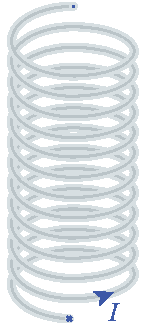
\includegraphics[width=0.5\textwidth]{images/chp8/chp8solenoide.pdf}
			\end{center}
		\end{minipage}
		\begin{minipage}{0.49\textwidth}
			\begin{center}
				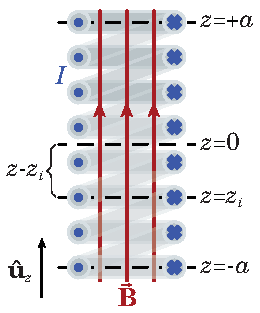
\includegraphics[width=1\textwidth]{images/chp8/chp8solenoidecrosssection.pdf}
			\end{center}
		\end{minipage}\\
		Nel caso qui raffigurato la corrente gira in senso antiorario. Per la regola della mano destra il campo prodotto da ciascuna spira del solenoide lungo l'asse è ortogonale e diretto verso l'alto; ci aspettiamo una sovrapposizione di tutti i campi vettoriali, intensificando il campo magnetico \textit{interno} complessivo.\\
		Il campo magnetico generato da una spira a quota $z_i$ in un punto lungo l'asse verticale a quota $z$ è, in modulo,
		\begin{equation*}
			\vba{B}_i=\frac{\mu_0 I R_0^2}{2\left(R_0^2+\left(z-z_i\right)^2\right)^{\nicefrac{3}{2}}}\vbh{u}_z
		\end{equation*}
		Il campo magnetico di un solenoide con $N$ spire è quindi
		\begin{equation*}
			\vba{B}=\sum_{i=1}^{N}\vba{B}_i
		\end{equation*}
		In molti casi, però, il numero di spire è talmente elevato che è molto più maneggevole passare al \textit{continuo}. Introducendo una densità \textit{lineare} $n$ di spire, ossia il numero di spire per unità di lunghezza, su un solenoide di lunghezza $2a$ si hanno
		\begin{equation*}
			N=\int_{-a}^{a}ndz
		\end{equation*}
		spire. Il campo magnetico infinitesimo ad altezza $z'$ si ottiene tenendo conto di quante spire ci sono nell'elemento di lunghezza $dz'$, ossia moltiplicando per la densità $n$ il campo magnetico infinitesimo che si avrebbe con una sola spira:
		\begin{equation*}
			d\vba{B}=\frac{\mu_0 I R_0^2 n}{2\left(R_0^2+\left(z-z'\right)^2\right)^{\nicefrac{3}{2}}}\vbh{u}_z\ dz'
		\end{equation*}
		Il campo magnetico complessivo si ottiene integrando lungo la lunghezza del solenoide. Supponendo che la densità di spire sia costante,
		\begin{equation*}
			B=\int_{-a}^{a}\frac{\mu_0 I R_0^2 n}{2\left(R_0^2+\left(z-z'\right)^2\right)^{\nicefrac{3}{2}}}\vbh{u}_z\ dz'=
			\frac{\mu_0 I n}{2R_0}\int_{-a}^{a}\frac{dz'}{\left(1+\frac{\left(z-z'\right)^2}{R_0^2}\right)^{\nicefrac{3}{2}}}\squarequal
		\end{equation*}
		Operando il campo di variabile $\eta=\dfrac{z'-z}{R_0}$, il differenziale diventa $d\eta=\dfrac{dz'}{R_0}$ mentre gli estremi di integrazione $\frac{\pm a-z}{R_0}$. Allora
		\begin{align*}
			\squarequal&\frac{\mu_0 I n}{2R_0}\int_{\frac{-a-z}{R_0}}^{\frac{a-z}{R_0}}\frac{\eta}{\left(1è\eta^2\right)^{\nicefrac{3}{2}}}=\frac{\mu_0 I n}{2}\eval{\frac{\eta}{\sqrt{1+\eta^2}}}_{\frac{-a-z}{R_0}}^{\frac{a-z}{R_0}}=\\
			=&\frac{\mu_0 I n}{2}\left(\frac{\frac{a-z}{R_0}}{\sqrt{1+\left(\frac{a-z}{R_0}\right)^2}}-\frac{\frac{a+z}{R_0}}{\sqrt{1+\left(\frac{a+z}{R_0}\right)^2}}\right)=
			\frac{\mu_0 I n}{2}\left(\frac{a-z}{\sqrt{R_0^2+\left(a-z\right)^2}}+\frac{a+z}{\sqrt{R_0^2+\left(a+z\right)^2}}\right)
		\end{align*}
		\begin{itemize}
			\item \textbf{In mezzo al solenoide} ($z=0$):
			\begin{equation}
				\vba{B}=\frac{\mu_0 I n a}{\sqrt{R_0^2+a^2}}\vbh{u}_z
			\end{equation}
			\item \textbf{Ad un estremo del solenoide} ($z=\pm a$):
			\begin{equation}
				\vba{B}=\frac{\mu_0 I n a}{\sqrt{R_0^2+4a^2}}\vbh{u}_z
			\end{equation}
			\item \textbf{Solenoide infinito} ($a\to+\infty$): il campo magnetico è omogeneo all'interno, pari a
			\begin{equation}
				\vba{B}=\mu_0 I n\vbh{u}_z
			\end{equation}
			e nullo all'esterno.
		\end{itemize}
		\begin{observe}
			Un solenoide infinito - nella pratica, un solenoide molto lungo - è un modo concreto per produrre un campo magnetico uniforme, costante e diretto verso l'alto.
		\end{observe}